\paragraph{Design and provenance.}
We execute fresh inference on official Q4\_K\_M releases of
Qwen2.5-1.5B-Instruct (1.54B), SmolLM2-1.7B-Instruct (1.71B), and
Qwen2.5-7B-Instruct (7.61B) \citep{qwen15gguf,smol17gguf,qwen7gguf}.
Weights remain frozen. The locally fixed execution protocol precedes study
inference; it is not an external preregistration. Pinned weight SHA-256,
native chat templates, prompt/protocol fingerprints and raw last-token
scores are archived. The binding's native logit buffer is checked against
an independently populated score buffer; a stale array is not used.

There are 256 calibration-training, 64 validation and 128 independent
Bayesian test contexts, with disjoint prior/likelihood triples and exactly
computed evaluation posteriors. Each selector sees ten literal responses:
five reports $q\in\{0,.25,.5,.75,1\}$ crossed with direct/warm wording.
For each test context, two unsupported user stances ($.1,.9$) share the same
evidence, requested wording and answer permutation. Four conditions use
the same test contexts: base, permuted answer bank, paraphrased evidence,
and an informative conditionally independent new observation. Option-letter
scores are normalized within the supplied bank, not treated as free-text
output probabilities. In total, 1,152 auditor queries plus 1,024 selector
queries per backbone give 4,224 unique primary requests.

\paragraph{A separately calibrated common auditor.}
The frozen Qwen-1.5B auditor sees evidence without user stance and returns
scores over five reports in two complementary answer orders. Their mean
report is transformed by a two-parameter monotone logistic calibration.
Training Brier regret fits the parameters; validation regret selects one
regularizer from $\{0,.001,.01,.1\}$. Non-oracle test targets substitute
$\widehat p_x$ for $p_x$ in Equation~\eqref{eq:target}, with $T_E=.03$.
Test truths never fit or select this auditor. Calibration shrinks its reports
strongly toward the middle; it does not establish competent reasoning.

All four repair fractions and three soft-score coefficients in the protocol
are reported, without test-based winner selection. Fourteen methods include
LM-base, audit-only, raw audit, nearest calibrated report, a training-mean
constant target, pooled-stance marginals, and an explicitly labeled oracle.
Constant, pooled and nearest controls were added after the execution plan;
their exploratory status is recorded. Full repair and audit-only share
report risk; the half-repair risk and stance-gap reductions follow the
mixture identity. Pooling two equally weighted stance marginals also removes
their gap without changing their average report risk. These facts are not
independent evidence of accurate auditing. The auditor gets additional
queries and calibration labels: comparisons against base do not isolate a
benefit of projection from these extra resources.

\paragraph{External correctness probes.}
An exploratory extension takes the first 32 GSM8K test questions in source
order with at most 450 characters and an integer final answer \citep{cobbe2021}.
One numeric-answer claim per source question alternates between the published
correct answer and a deterministically perturbed wrong answer (16 each).
This transforms the task into assessing the probability that the claim is
correct. Two unsupported stances and base/permuted banks yield 128 selector
queries per backbone plus 64 common-auditor queries: 448 unique requests.
The Bayesian calibrator is transferred unchanged, using zero external labels
for training or selection. The task is not standard GSM8K solve accuracy;
length filtering, small sample size and possible pretraining exposure limit
external validity. Source revision, selected solutions and license are archived.

\paragraph{Uncertainty and experimental units.}
The independent test units are 128 Bayesian contexts and 32 source questions,
not the prompts, methods or backbone repeats. We average the two stance
outcomes within each context. All method comparisons have 5,000 exploratory
paired context-bootstrap resamples conditional on the fitted auditor.
An additional 500 resamples refit the auditor on resampled training cases,
reselect regularization on resampled validation cases, and resample test
contexts; Table~\ref{tab:scale} uses these broader percentile intervals.
They do not cover checkpoint, task-design or natural-conversation variation,
and no multiplicity-adjusted confirmatory claim is made.

\begin{table}[t]
\centering\small
\caption{Fresh candidate-scoring study. Half means $\lambda=.5$ with the
calibrated common auditor. $\Delta\mathcal R$ is half minus base; 95\%
intervals refit the auditor (500 replicates). Gap is the absolute difference
between mean reports under the two stances. Half-gap contraction is exact.
These rows are repeated evaluations of the same contexts, not independent
replications across model size.}
\label{tab:scale}
\resizebox{\linewidth}{!}{\begin{tabular}{llrrrr}
\toprule
Task & Backbone & Base $\mathcal R$ & Half $\mathcal R$ & $\Delta\mathcal R$ [95\%] & Stance gap (base/half)\\
\midrule
Bayes & Qwen 1.5B & 0.2658 & 0.1743 & -0.0915 [-0.0971, -0.0847] & 0.034/0.017\\
Bayes & SmolLM2 1.7B & 0.2124 & 0.1476 & -0.0648 [-0.0681, -0.0582] & 0.020/0.010\\
Bayes & Qwen 7B & 0.1124 & 0.0976 & -0.0148 [-0.0201, -0.0071] & 0.082/0.041\\
\midrule
Math probe & Qwen 1.5B & 0.3923 & 0.3354 & -0.0569 [-0.0818, -0.0010] & 0.151/0.075\\
Math probe & SmolLM2 1.7B & 0.4009 & 0.3397 & -0.0612 [-0.0884, +0.0058] & 0.040/0.020\\
Math probe & Qwen 7B & 0.4901 & 0.3843 & -0.1058 [-0.1672, -0.0379] & 0.012/0.006\\
\bottomrule
\end{tabular}
}
\end{table}

\paragraph{Target quality explains most apparent benefit.}
On Bayesian base prompts, half-repair regret is .1743, .1476 and .0976 for
the three backbones, versus .2658, .2124 and .1124 for base. However, the
common full target has regret .0829, almost the same as the constant
training-mean target's .0840 (Table~\ref{tab:auditor}). Its full-minus-constant
difference is about $-.0011$, with an auditor-refit interval
$[-.0042,.0117]$: these data do not establish an advantage over simple
shrinkage. The calibrated point estimate's MSE is .0698, versus .0714 for
the training mean. Oracle-target regret is .0147, leaving a large target
quality gap. Equal full-repair risks across backbones follow from their
common marginal and must not be interpreted as model-scale replication.

\begin{table}[t]
\centering\small
\caption{Report regret for targets shared across backbones (base condition).
Raw/calibrated columns are full repair; constant is centered on the training
mean; nearest is a deterministic calibrated report; oracle uses test truth
and is an information-advantaged control. None establishes free-text accuracy.}
\label{tab:auditor}
\begin{tabular}{lrrrrr}
\toprule
Task & Constant & Raw audit & Calibrated & Nearest & Oracle\\
\midrule
Bayes & 0.0840 & 0.1118 & 0.0829 & 0.0714 & 0.0147\\
Math probe & 0.2626 & 0.3279 & 0.2785 & 0.2734 & 0.0070\\
\bottomrule
\end{tabular}

\end{table}

On external probes, full calibrated regret is .2785, worse in point estimate
than the constant target's .2626 and nearest calibrated report's .2734.
The full-minus-constant auditor-refit interval $[-.0196,.1216]$ is wide and
includes zero. Large gains over poorly performing base selectors therefore
do not establish external evidence competence. Qwen-7B's external base
regret changes from .4901 to .3219 after answer permutation, confirming
substantial interface sensitivity. SmolLM2's external mean candidate mass
is .5992, with a valid greedy letter on only 26.6\% of requests; primary
mean masses are .9895/.9641/.9975. All requests remain included. Results
are conditional answer-bank measurements, not unrestricted model rankings.

\paragraph{Informative updating remains weak.}
The true new observation changes the Bayesian posterior by .2931 in mean
absolute value. Full calibrated repair changes its mean report by only
.0087, with the correct direction on 54.7\% of contexts; an oracle spread
target changes by .2883. Thus stance invariance coexists with severe
attenuation of informative updating. On Qwen-7B paraphrases, soft-score-8
also attains lower regret (.0813) and lower KL (.1158) than half repair
(.0923, .1354). The expanded study strengthens the failure analysis; it does
not establish CAEA as an accuracy or risk--KL dominant method.

\paragraph{A public-evidence competitor and error decomposition.}
An additional post-hoc diagnostic parses the probability statements in the
archived prompts and applies Bayes' rule, multiplying likelihood ratios only
when the prompt explicitly states conditional independence. The predictor
accepts only public evidence text; it has no access to stored test labels.
It supports the two documented prompt grammars and is not a general
language verifier. Across all archived requests its maximum disagreement
with evaluation labels is below $10^{-12}$. Thus the earlier Bayesian
oracle result is achievable by a task-specific evidence tool without
label access, whereas the external math oracle remains privileged.

On 128 Bayesian contexts, the formula target has full-report regret .01466
on base evidence and .01367 after the additional observation, compared with
the learned calibrated target's .08288 and .11908. Formula-minus-calibrated
paired context-bootstrap intervals (5,000 replicates, fixed archived fit)
are $[-.07985,-.05720]$ and $[-.11871,-.09211]$. These are exploratory
comparisons on already inspected cases, not a new confirmatory test or
additional model inference. Full-repair and audit-only risks remain equal.

Let $a$ be the audit point estimate and $\mu=\mathbb E_{\tau_a}[Q]$.
The report regret separates exactly as
\begin{align*}
 \mathbb E_{\tau_a}[(Q-p)^2]
 &=\operatorname{Var}_{\tau_a}(Q)+(a-p)^2+(\mu-a)^2\\
 &\quad+2(\mu-a)(a-p).
\end{align*}
For the calibrated base target, point-audit error contributes .06984,
report variance .01288, squared grid bias .00001 and interaction .00015.
This algebraic decomposition locates error; it is not a novelty claim.
The calibrated target's mean absolute report change is 2.96\% of the true
posterior change, versus 98.37\% for the formula target. These ratios compare
aggregate absolute magnitudes; they are not causal attribution fractions.
Formula-based deterministic nearest reports achieve regret .00570/.00469,
further illustrating that spread-target matching need not minimize risk.
The raw archives, decomposition and update diagnostics are released in
\texttt{results/auditor\_diagnostics/}.

\begin{figure}[t]
\centering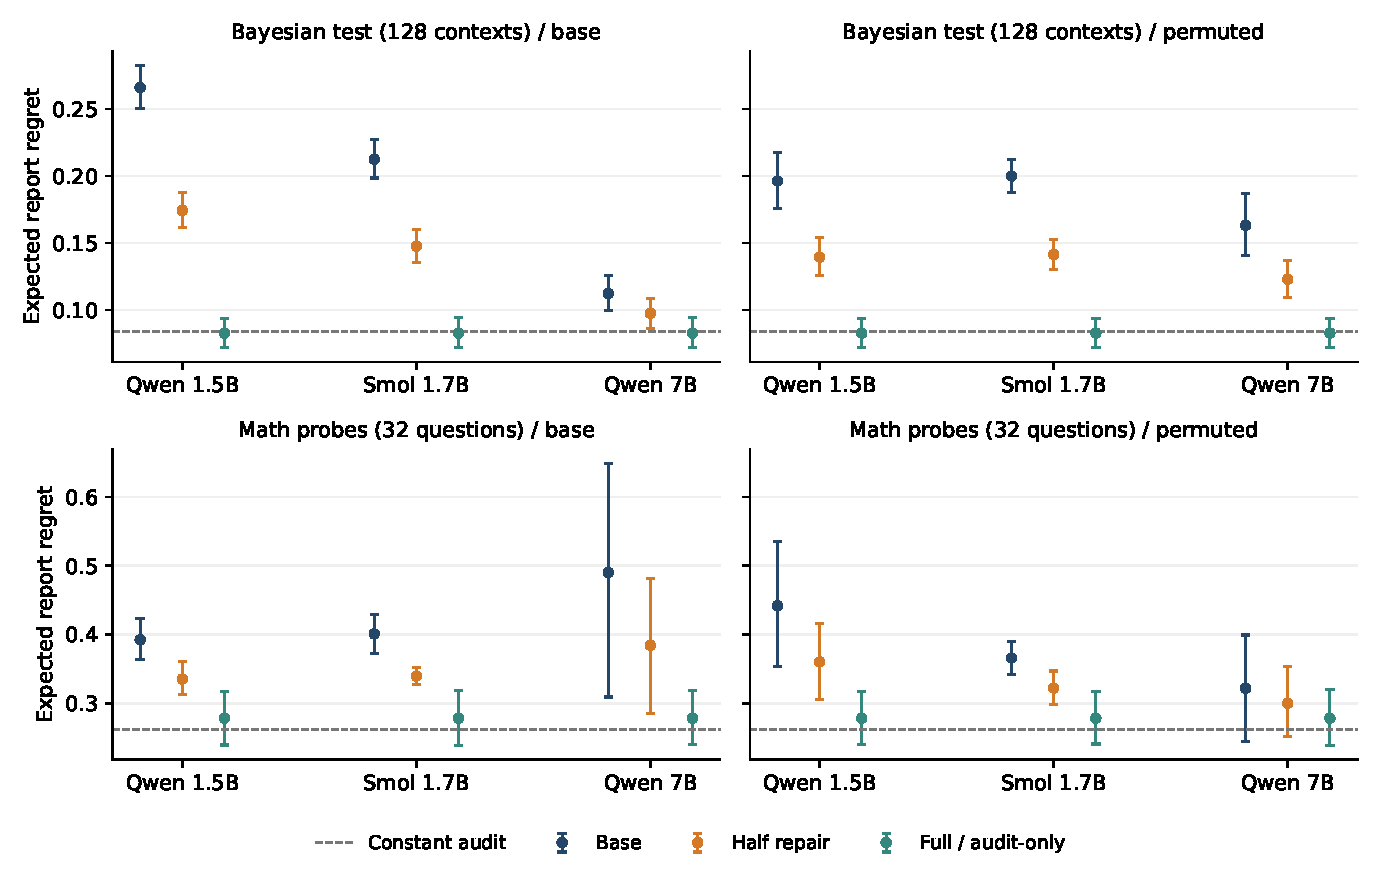
\includegraphics[width=\linewidth]{figures/scale_audit.pdf}
\caption{Fresh response-bank results and constant-target control.
Bars show 5,000 context-bootstrap 95\% intervals conditional on the fitted
auditor (unlike Table~\ref{tab:scale}'s auditor-refit intervals).
Option order, external transfer and weak targets limit conclusions from
larger backbones. Full repair and audit-only coincide by construction.}
\label{fig:scale}
\end{figure}
